\section*{Phenomenon Description}

A voting system takes as input a collection of individual preference rankings and produces a single collective outcome. Each voter submits a total ordering of the available options, specifying a strict sequence from most to least preferred, without ties. The voting rule processes these inputs and returns either a single winner or a complete ranking of the options according to the aggregated preferences.

These systems formalize the process of collective decision-making. Their applications extend beyond political elections and include committee procedures, academic appointments, boardroom voting, and algorithmic decision-making in multi-agent systems and recommendation engines.

Mathematically, the input to a voting system is called a profile: a multiset of total orders, with one such order for each voter. Each total order ranks the finite set of alternatives such that every candidate is assigned a unique position. This representation provides the raw structure on which aggregation rules operate.

The number of possible total orderings grows rapidly with the number of options. For three candidates, there are $3! = 6$ distinct rankings; for five candidates, there are $5! = 120$. This factorial growth introduces combinatorial complexity, making it infeasible to analyze all possible configurations exhaustively once the number of alternatives exceeds a small threshold.

Certain structural properties are often desired of voting rules. Anonymity requires that the outcome not depend on which voter submitted which ballot. Neutrality requires that all candidates be treated symmetrically. These properties enforce formal symmetries on the rule and ensure that it operates independently of irrelevant identifiers.

Additional desirable properties include monotonicity and consistency. A system is monotonic if ranking a candidate higher on a ballot cannot reduce that candidate’s chances of winning. It is consistent if identical outcomes from separate groups imply the same outcome when those groups are merged. These properties aim to prevent procedural anomalies that would violate intuitive fairness.

Several voting systems are widely implemented in practice. These include plurality voting, the Borda count, Condorcet methods, and instant-runoff voting. Each of these systems interprets the profile differently and emphasizes different structural aspects of the ranking data.

Plurality voting considers only the top-ranked candidate on each ballot. The candidate receiving the most first-place votes is declared the winner. All lower-ranked information is discarded, making the system computationally simple but highly sensitive to strategic voting and vote splitting.

The Borda count assigns a score to each candidate based on their rank position on each ballot. For example, in a three-candidate election, a first-place vote may yield two points, second place one point, and third place zero. These points are then summed across all ballots, and the candidate with the highest total score wins. This method incorporates more information from the ranking but can fail to elect a candidate who would beat all others in head-to-head contests.

Condorcet methods use pairwise majority comparisons between candidates. For each pair, the number of voters who prefer one candidate to the other is counted. If a candidate defeats every other candidate in these head-to-head contests, that candidate is called the Condorcet winner. Not all profiles contain such a candidate, and additional rules are required when cycles occur.

Instant-runoff voting proceeds through iterative elimination. In each round, the candidate with the fewest first-place votes is eliminated, and those ballots are reassigned to the next preferred remaining candidate. The process continues until a single candidate remains. This system allows voters to express multiple preferences but can still produce paradoxical reversals when a candidate gains additional support.

Each of these methods can produce different results on the same input profile. The choice of rule determines which structural features of the preferences are preserved and which are ignored. No method fully captures all intuitively fair principles, and the differences between them reflect the trade-offs inherent in social choice.

\begin{table}[H]
\centering
\renewcommand{\arraystretch}{1.25}
\begin{tabular}{l|ccc}
\textbf{Voter} & \textbf{1st choice} & \textbf{2nd choice} & \textbf{3rd choice} \\
\hline
1 & A & B & C \\
2 & A & B & C \\
3 & B & C & A \\
4 & B & C & A \\
5 & C & A & B \\
\end{tabular}

\vspace{1em}

\begin{tabular}{l|l}
\textbf{Voting Method} & \textbf{Winner} \\
\hline
Plurality (most 1st-place votes) & Tie: A, B (2 votes each) \\
Borda Count (2–1–0 scoring) & B (6 points) \\
Condorcet (pairwise majority) & No winner (cycle: A→B→C→A) \\
Instant-Runoff & A (C eliminated, votes transfer to A) \\
\end{tabular}
\caption{Different voting methods yield different winners from the same preferences.}
\end{table}

The existence of divergent outcomes reveals a fundamental ambiguity: no canonical method summarizes multiple rankings into a single decision. Each method prioritizes different structural information.

Even if all voters submit transitive rankings, the group preference can form a cycle. A common instance involves three voters and three candidates, each favored in a rotating fashion:

\begin{figure}[H]
\centering
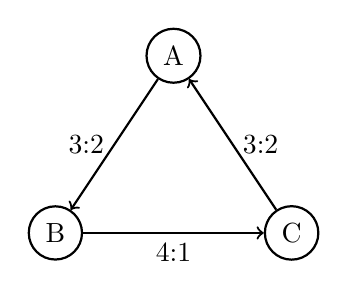
\begin{tikzpicture}[scale=1.5, ->, thick]
\node[circle, draw] (A) at (0,1) {A};
\node[circle, draw] (B) at (-1,-0.5) {B};
\node[circle, draw] (C) at (1,-0.5) {C};
\draw (A) -- (B) node[midway, left] {3:2};
\draw (B) -- (C) node[midway, below] {4:1};
\draw (C) -- (A) node[midway, right] {3:2};
\end{tikzpicture}
\caption{Condorcet cycle: A beats B, B beats C, C beats A, showing majority preference cycles even when individual voters rank consistently.}
\end{figure}


Cycles in group preferences arise even when individual preferences are fully ordered and consistent. Each voter's ballot may assign a strict ranking to all options, but the collective result may still fail to satisfy transitivity. For example, candidate A may be preferred to B by a majority, B preferred to C, and yet C preferred to A, forming a cycle. This outcome cannot be mapped to a total order and reveals a limitation that no voting rule can avoid in all cases.

Any system that outputs a full group ranking must address such cycles. One approach is to discard some pairwise comparisons and resolve the ranking using the remaining ones. Another approach is to introduce external tie-breaking rules, which may depend on arbitrary or external criteria. Both strategies impose coherence on an input that may not support it.

Kenneth Arrow proposed a precise framework to evaluate the reasonableness of voting systems. He identified four conditions that any acceptable aggregation rule might aim to satisfy: unanimity, non-dictatorship, independence of irrelevant alternatives, and transitivity.

Unanimity requires that if all voters rank option $X$ above option $Y$, then the group outcome must reflect that same order. Non-dictatorship ensures that no single voter can always determine the result regardless of the others' preferences. These two conditions express responsiveness and fairness.

The third condition, independence of irrelevant alternatives (IIA), states that the group preference between any two options $X$ and $Y$ should depend only on how voters rank $X$ relative to $Y$. Preferences involving other options must not affect the outcome of this pairwise comparison. This condition ensures that unrelated rankings cannot distort local outcomes.

Transitivity requires consistency across comparisons: if the group prefers $X$ to $Y$ and $Y$ to $Z$, it must also prefer $X$ to $Z$. If transitivity fails, the output cannot be interpreted as a ranking at all — it contains loops that prevent any ordering from being formed.

Arrow’s impossibility theorem proves that no method satisfies all four conditions — unanimity, non-dictatorship, IIA, and transitivity — when there are at least three options and at least two voters. This is not a limitation of particular procedures. It is a general result that rules out the possibility of combining all these demands at once.

The conclusion is not that voting is invalid, but that trade-offs are unavoidable. Some methods give up IIA to maintain collective agreement and equal treatment of voters. Others allow intransitive outcomes in order to preserve independence or avoid concentrated control. Every system must fail at least one of the criteria.

Later interpretations describe rankings as points in a space of permutations. A profile, consisting of all voters’ rankings, becomes a set of such points. This point of view makes it possible to treat voting rules as functions from profiles to outcomes.

Each condition corresponds to a constraint on the aggregation function: it must treat voters and options equally, rely only on relevant comparisons, and produce a transitive outcome. No function can satisfy all of these constraints at once. Even when every criterion seems reasonable in isolation, their combination fails when applied to rankings from multiple voters. Arrow’s theorem shows that this conflict cannot be avoided across all possible inputs.

\begin{commentary}[Mathematics Beyond Physics]
I included this chapter to demonstrate that mathematical limitations, though typically associated with physical systems, can sometimes apply to social processes as well.

As an undergraduate, I took courses in game theory given by Ron Holzman, who has Erdős number 1 for a paper on maximal triangle-free graphs (where any added edge creates a triangle).

Ron also co-authored, in 2001 with Tom Bohman and Dan Kleitman, a proof of the $n = 6$ case of the Lonely Runner Conjecture. This conjecture states that for any $n$ runners moving at constant but distinct speeds around a circular track of unit length, there exists a time when each runner is at least $1/n$ of the track away from every other runner. The problem models the moment when, despite all runners moving continuously and independently, each one is "lonely" — meaning far enough from all others to be considered isolated.

I loved this problem because the cases $n = 2$ and $n = 3$ are easy to visualise and prove (albeit lengthy for $n = 3$) using elementary arguments, yet the general case has resisted a full proof for over fifty years. It is currently known only for $n \leq 7$.

The conjecture has an elegant reformulation in terms of number theory and approximation on the unit circle. For a runner moving at integer speed $v$, define the Bohr set $B(v,\delta) = \{ t \in \mathbb{R}/\mathbb{Z} : \|vt\| \leq \delta \}$, where $\|x\|$ denotes the distance from $x$ to the nearest integer. This set consists of all times when the runner is within a distance $\delta$ of their starting point.

Then, for distinct non-zero integer speeds $v_1, \dots, v_n$, define $\delta(v_1, \dots, v_n)$ to be the smallest $\delta$ such that the union of the Bohr sets $B(v_i, \delta)$ covers the entire circle. The Lonely Runner Conjecture is equivalent to the claim that for any such tuple, $\delta(v_1, \dots, v_n) \geq 1/(n+1)$, and that this bound is tight.

In this formulation, the conjecture becomes a covering problem for subsets of the torus, and connects to Diophantine approximation and additive combinatorics. The difficulty is in showing that the runners cannot remain clustered indefinitely, even when moving at completely different rates. Despite several partial results and asymptotic bounds, no general proof is known, and improving even the trivial union bound remains a significant challenge.

That such a question — about runners on a track — can be rephrased in terms of fractional parts, Bohr sets, and the geometry of coverings in $\mathbb{R}/\mathbb{Z}$ illustrates how problems from everyday intuition often touch the edge of what mathematics can currently answer.
\end{commentary}


\begin{figure}[H]
\centering
\begin{tikzpicture}[scale=1.2, >=Stealth]

  % Helper to draw runner with arrow
  \newcommand{\runnerarrow}[2]{%
    \draw[->, thick] (#1:1) ++({cos(#1+90)*0.05},{sin(#1+90)*0.05}) -- ++({cos(#1+90)*0.2},{sin(#1+90)*0.2});
    \fill[black] (#1:1) circle (0.03);
    \node at (#1:1.25) {\tiny #2};
  }

  % N = 2
  \begin{scope}[shift={(-4,0)}]
    \draw[thick] (0,0) circle (1);
    \runnerarrow{0}{R1}
    \runnerarrow{180}{R2}
    \node at (0,-1.3) {\footnotesize $n = 2$};
  \end{scope}

  % N = 3
  \begin{scope}
    \draw[thick] (0,0) circle (1);
    \runnerarrow{0}{R1}
    \runnerarrow{120}{R2}
    \runnerarrow{240}{R3}
    \node at (0,-1.3) {\footnotesize $n = 3$};
  \end{scope}

  % N = 4
  \begin{scope}[shift={(4,0)}]
    \draw[thick] (0,0) circle (1);
    \runnerarrow{0}{R1}
    \runnerarrow{90}{R2}
    \runnerarrow{180}{R3}
    \runnerarrow{270}{R4}
    \node at (0,-1.3) {\footnotesize $n = 4$};
  \end{scope}

\end{tikzpicture}

\caption{\textit{The Lonely Runner Conjecture for $n = 2$, $3$, and $4$. Each circle shows a time when every runner is at least $1/n$ of the track away from all others. Arrows indicate the direction of motion.}}
\end{figure}

\begin{SideNotePage}{
  \textbf{Top — Voting Methods:} \par Ranked-choice voting is a system in which voters express their preferences by submitting complete rankings of all candidates, and the system aggregates them into a ranked list or a single winner. Different aggregation methods (Borda count, IRV, Plurality, Condorcet) can produce distinct winners from identical voter rankings, demonstrating the inherent ambiguity in collective decision-making. The same preference profile can yield different outcomes depending on which structural aspects of the rankings are emphasized by the chosen method. This fundamental indeterminacy reveals that there is no canonical way to translate individual preferences into collective choices.

  \vspace{1.5em}
  \textbf{Bottom — Arrow's Theorem:} \par Arrow's impossibility theorem proves that no ranked-choice voting method can satisfy all four fairness criteria simultaneously when there are at least three alternatives and two voters: 1) no dictatorship (no single voter controls all outcomes), 2) Pareto unanimity (universal agreement is respected), 3) independence of irrelevant alternatives (pairwise rankings unaffected by third options), 4) completeness and transitivity (coherent group rankings). Every democratic aggregation method must compromise at least one criterion, making trade-offs unavoidable in social choice. This mathematical limitation applies to all possible voting systems, not just those currently in use.
}{09_ArrowTheoremTopology/UNPOPSCI - DEMOCRACY - vF.pdf}
\end{SideNotePage}
